\chapter{Resultados}
%\markboth{\thechapter ~~~ Resultados}{}
%\label{result}

Neste capítulo, os resultados para o projeto descritos no capítulo anterior serão apresentados. A obtenção do modelo da 
planta foi dada de duas formas diferentes: através da convenção de \textit{Denavit-Hartenberg} e equações de 
\textit{Euler-Lagrange} e através do ensaio em malha aberta. Para o primeiro método, foram feitas algumas considerações,
estas seguem abaixo:

\begin{enumerate}
 \item O elo do cotovelo e o elo do ombro são barras de comprimento $L$ e massa $m$, e possuem o eixo de rotação no fim
 da barra;
 \item O elo da base é um cilindro sólido de raio $r$, altura $h$ e massa $m$;
 \item A distribuição de massa de cada elo com a sua junta respectiva é simétrica em relação à estrutura do corpo. Ou seja,
 a massa está uniformemente distribuída ao longo do corpo.
\end{enumerate}

A modelagem através da convenção de \textit{Denavit-Hartenberg} e equações de \textit{Euler-Lagrange} foi feita de forma
programática através do MATLAB e segue no \refanexo{anexo:denHatEulerLagr}. Os modelos da planta usados para projetar os
constroladores foram obtidos através do ensaio em malha aberta e seguem na próxima seção. Três modelos foram levantados,
um para a base, um para o ombro e outro para o cotovelo, e para cada um deles foi projetado um controlador, esse 
processo é conhecido na literatura como controle de juntas independentes.

\section{Ensaio em malha aberta}
\markright{\thesection ~~~ Resultado ensaio em malha aberta}

A comunicação com os servomotores foi feita inicialmente com um computador através da porta serial com o protocolo 
\textit{UART}. A linguagem usada para a execução do ensaio em malha aberta foi o \textit{python}, e seu código completo
encontra-se em \cite{lelis_model}.

Para cada uma das juntas, foi feita uma montagem semelhante à \autoref{fig:diagEnsaioMA}. Foi aplicada na entrada de
cada um dos servos uma referência em degrau para o ângulo $\theta$ ($^\circ C$). Inicialmente, o sistema tinha sido
configurado para uma amostragem de $0,01s$, de acordo com a resposta obtida, observou-se uma superamostragem dos dados,
com isso, o tempo de amostragem foi alterado para $0,23s$. As saídas $\theta$ ($^\circ C$) obtidas
ao longo do tempo seguem na \autoref{fig:ensaioMalhaAberta}.

\begin{figure}[h!]
  
  \centering
  \caption{Gráficos da entrada e resposta para o ensaio em MA de cada uma das juntas}
  \begin{subfigure}{.5\textwidth}
    \centering
    \caption{Base}
    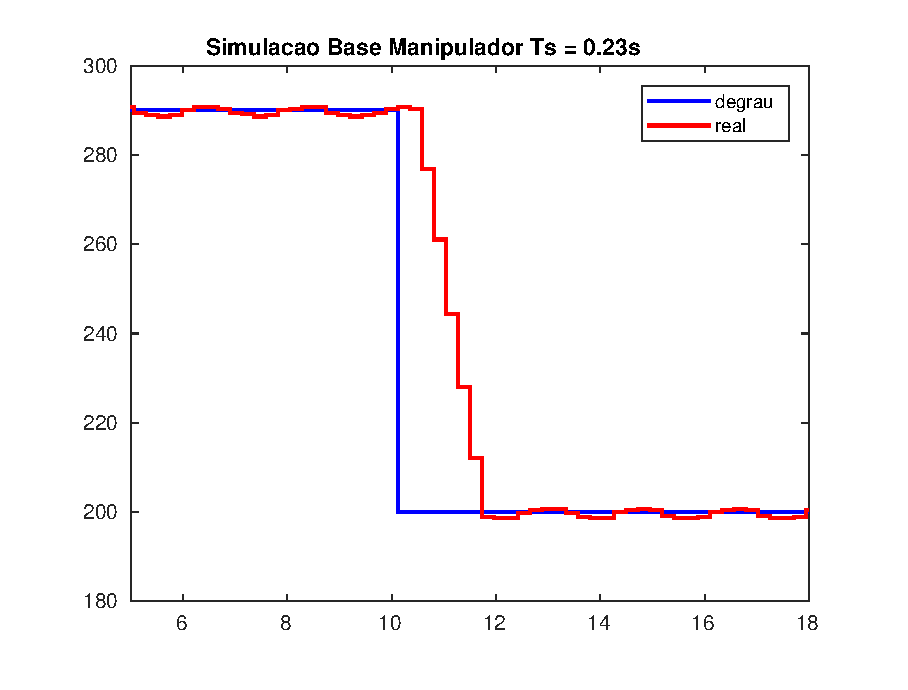
\includegraphics[width = 1\columnwidth]{Imagens/base_ma}
    \fonte{Do autor}
    \label{fig:base_ma}
  \end{subfigure}%
  \begin{subfigure}{.5\textwidth}
    \centering
    \caption{Ombro}
    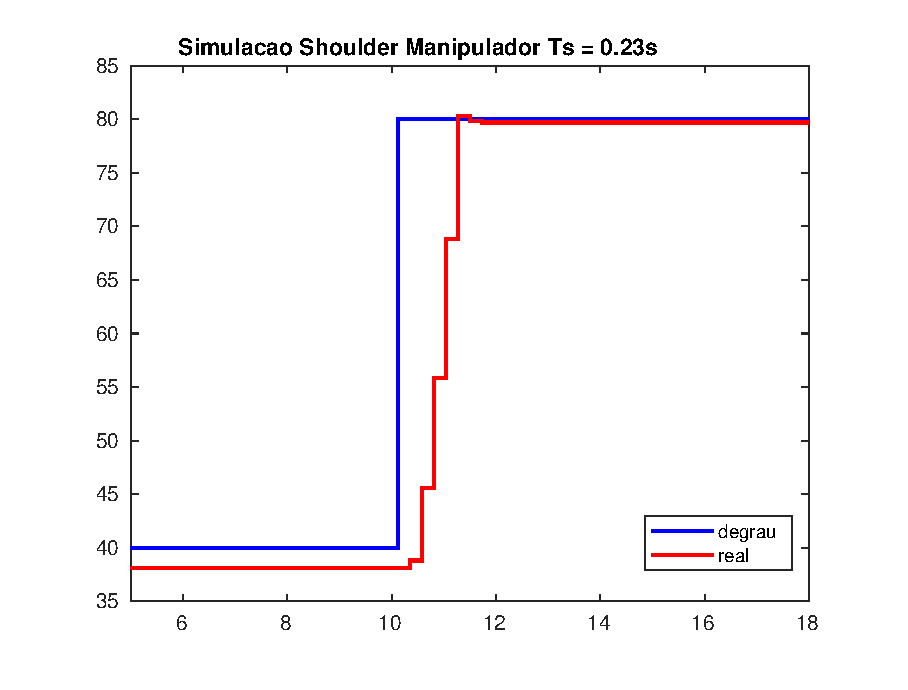
\includegraphics[width = 1\columnwidth]{Imagens/shoulder_ma}
    \fonte{Do autor}
    \label{fig:shoulder_ma}
  \end{subfigure}%
  \\[5ex]
  \begin{subfigure}{\textwidth}
    \centering
    \caption{Cotovelo}
    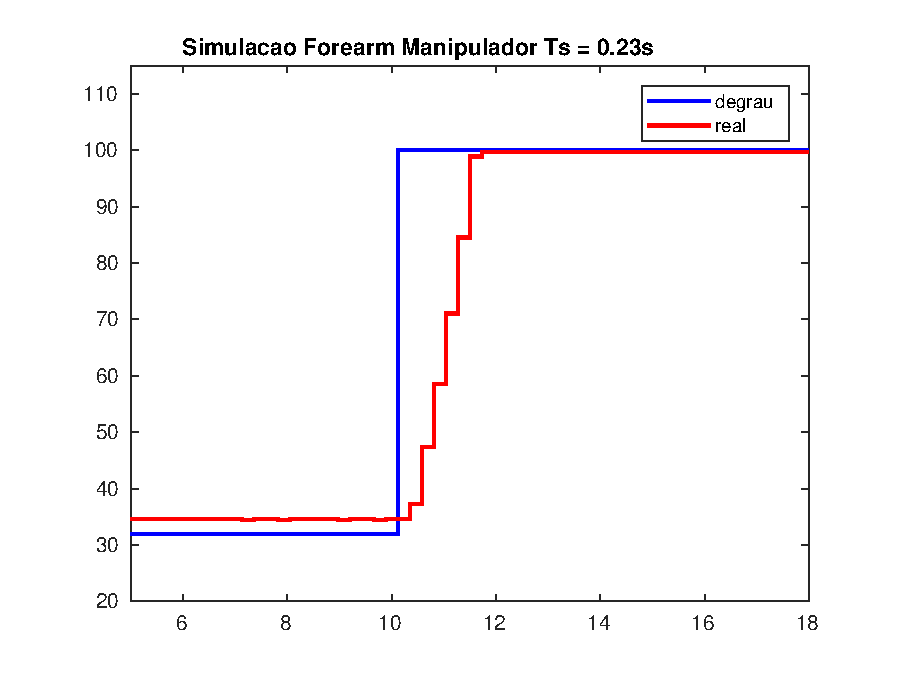
\includegraphics[width = 0.55\columnwidth]{Imagens/forearm_ma}
    \fonte{Do autor}
    \label{fig:forearm_ma}
  \end{subfigure}%
  
  \label{fig:ensaioMalhaAberta} 

\end{figure}

O modelo de cada junta poderia ser aproximado para uma modelo de primeira ordem, mas os servomotores possuem
um controlador interno de configuração eletrônica para o ângulo. Por esse motivo, o mais apropriado foi 
aproximar cada junta para um modelo de segunda ordem, conforme \eqref{eq:sistemaSegundaOrdem}.

Observando as Figuras \ref{fig:base_ma} e \ref{fig:forearm_ma}, observa-se um comportamento próximo do 
amortecimento crítico. Quando ocorre esse tipo de comportamento, pode-se fazer a 
aproximação: $\xi = 1$ \cite{Ogata}, \cite{Castrucci}. Por outro lado, em \ref{fig:shoulder_ma}, observa-se
um pequeno sobressinal, o que resulta em um $\xi$ menor, aproximando-se para este caso: $\xi = 0,8$.

O tempo de acomodação, definido em \eqref{eq:tempoAcomodacao}, variou para todas as juntas uma quantidade
semelhante $0,9s < t_s < 1,3s$. De acordo com testes visuais para a validação do modelo, e pelas Figuras 
\ref{fig:base_ma}, \ref{fig:shoulder_ma} e \ref{fig:forearm_ma}, foi considerado para a base, ombro e
cotovelo respectivamente: $t_s = 1,0952s$, $t_s = 0,9333s$, $t_s = 1,0952s$. Dessa forma, substituindo em 
\eqref{eq:tempoAcomodacao} as constantes encontradas por aproximação, obtém-se para o $\omega_n$ da base, ombro e
cotovelo respectivamente: $\omega_n = 3.6522 rad/s$, $\omega_n = 5.3571 rad/s$, $\omega_n = 3.6522 rad/s$.
O valor das variáveis encontradas para cada uma das juntas segue na \autoref{tab:ctesModeloMA}

\begin{center}
    \captionof{table}{Constantes encontradas para o modelo de segunda ordem}
    \begin{tabular}{| c | c | c | c |}\hline
      \textbf{Junta}	& $\xi$ 	& $t_s$ (s)	& $\omega_n$ (rad/s)	\\ \hline
      Base		& 1 		& 1,0952	& 3,6522		\\ \hline
      Ombro		& 0,8 		& 0,9333	& 5,3571		\\ \hline
      Cotovelo		& 1 		& 1,0952	& 3,6522		\\ \hline
    \end{tabular}
    \label{tab:ctesModeloMA}
\end{center}

\section{Fase 1 da técnica HIL}
\markright{\thesection ~~~ Fase 1 da técnica HIL}

Como foi exposto na seção anterior, as constantes foram encontradas por aproximações de acordo
com o que foi observado no ensaio em malha aberta. A partir disso, as funções de transferência
para a base, ombro e cotovelo foram obtidas através da \autoref{eq:sistemaSegundaOrdem} e 
seguem respectivamente em \eqref{eq:baseModel}, \eqref{eq:shoulderModel} e \eqref{eq:forearmModel}:

\begin{equation}
  \begin{gathered}
    G(s) = \frac{13,3384}{s^2 + 7,3043s + 13,3384}
  \end{gathered}
  \label{eq:baseModel}
\end{equation}

\begin{equation}
  \begin{gathered}
    G(s) = \frac{0,9965 \cdot 28,69898}{s^2 + 8,5714s + 28,69898}
  \end{gathered}
  \label{eq:shoulderModel}
\end{equation}

\begin{equation}
  \begin{gathered}
   G(s) = \frac{13,3384}{s^2 + 7,3043s + 13,3384}
  \end{gathered}
  \label{eq:forearmModel}
\end{equation}

As funções de transferência obtidas representam uma simulação da planta do projeto.
O mesmo degrau aplicado na planta real, foi aplicado nas funções de transferência para
a validação dos modelos. Os resultados obtidos seguem na \autoref{fig:base_ma_simul}, 
\ref{fig:shoulder_ma_simul} e \ref{fig:forearm_ma_simul}.

\begin{figure}[h!]
  
  \centering
  \caption{Gráficos da entrada e resposta do modelo obtido para cada uma das juntas}
  \begin{subfigure}{.5\textwidth}
    \centering
    \caption{Base}
    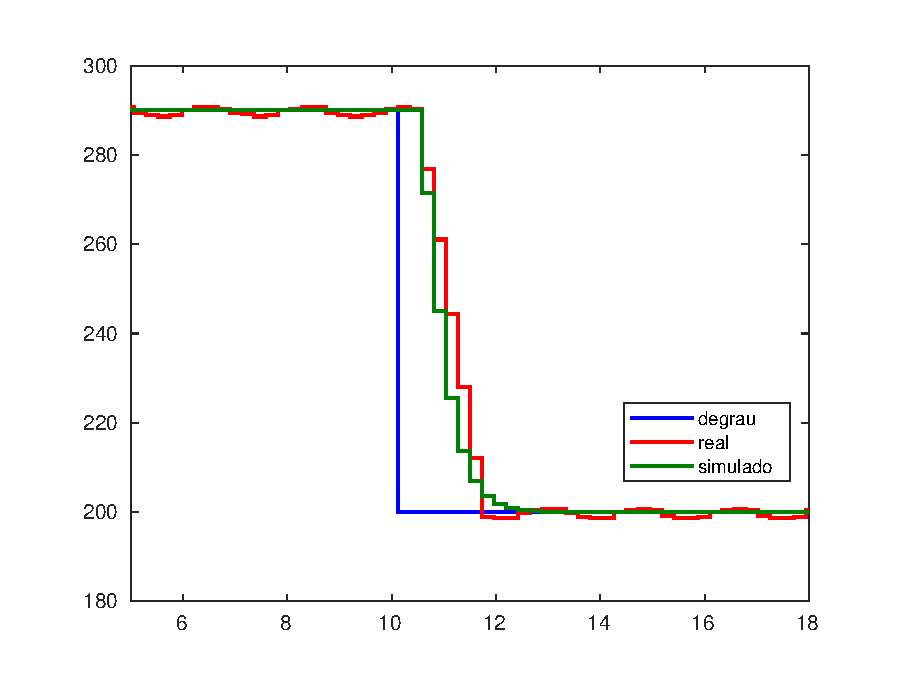
\includegraphics[width = 1\columnwidth]{Imagens/base_ma_simul}
    \fonte{Do autor}
    \label{fig:base_ma_simul}
  \end{subfigure}%
  \begin{subfigure}{.5\textwidth}
    \centering
    \caption{Ombro}
    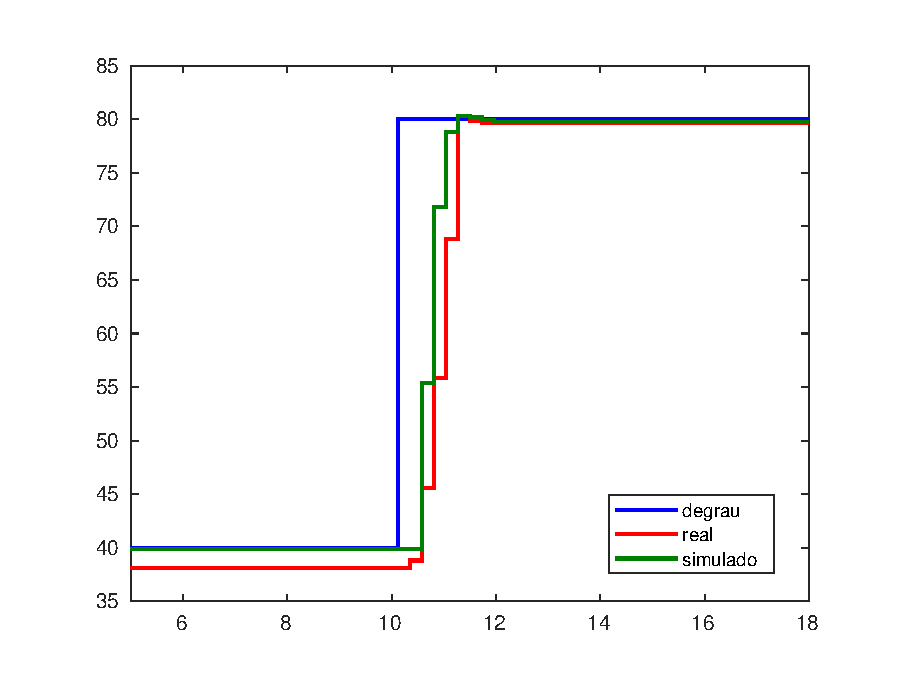
\includegraphics[width = 1\columnwidth]{Imagens/shoulder_ma_simul}
    \fonte{Do autor}
    \label{fig:shoulder_ma_simul}
  \end{subfigure}%
  \\[5ex]
  \begin{subfigure}{\textwidth}
    \centering
    \caption{Cotovelo}
    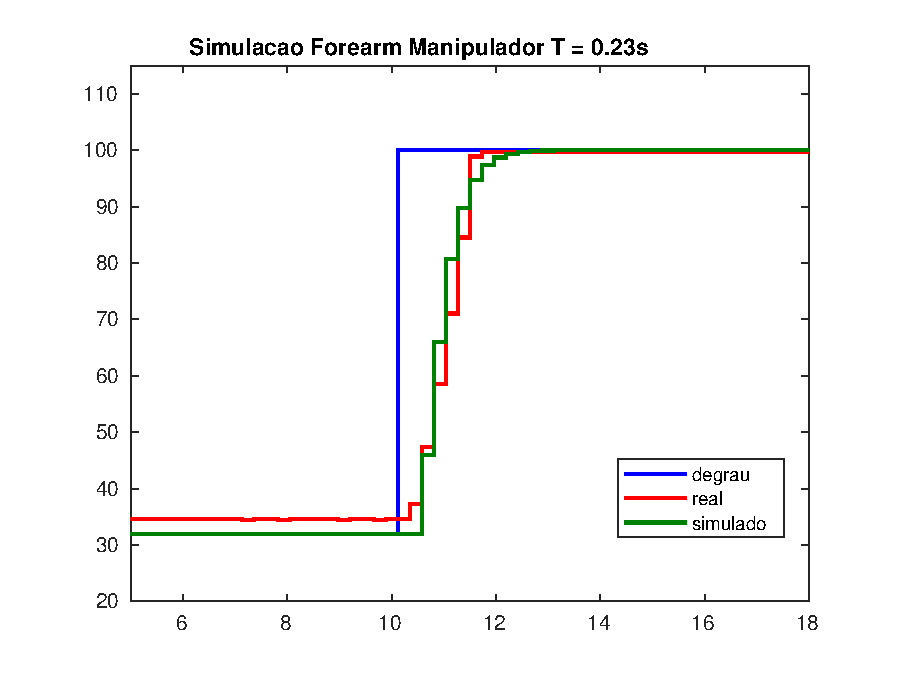
\includegraphics[width = 0.55\columnwidth]{Imagens/forearm_ma_simul}
    \fonte{Do autor}
    \label{fig:forearm_ma_simul}
  \end{subfigure}%
  
  \label{fig:ensaioMalhaAberta} 

\end{figure}

Obtidos os modelos, a próxima etapa da fase 1 da técnica HIL foi o projeto dos 
controladores pelo método do lugar das raízes. Considerando que as especificações do projeto
de controle seriam atendidas caso houvesse pouco sobressinal na resposta, e o erro em estado
estacionário igual a zero, mesmo impactando negativamente no tempo de acomodação, um controlador 
PI para cada junta seria suficiente. O controlador PI corresponde a \autoref{eq:pid} sem a ação 
derivativa. Assim sendo, na análise do lugar das
raízes (através da ferramenta \textit{sisotool} do \textit{Matlab}), foi colocado um polo de malha
fechada na origem e um zero no eixo real para o controlador de cada uma das juntas. O ganho foi 
ajustado de tal forma que os polos de malha fechada ficassem o mais próximo possível do eixo real, 
assim a resposta não apresentaria oscilação (ou quase não apresentaria) ao fechar a malha. Outra 
consideração importante observada foi modelar o controlador de tal forma que mesmo depois da 
discretização, ele não apresentasse zeros não mínimos. O resultado final obtido para os controladores 
da base, ombro e cotovelo seguem respsectivamente em \eqref{eq:base_ctrl}, \ref{eq:shoulder_ctrl}
e \ref{eq:forearm_ctrl}:

\begin{equation}
  \begin{gathered}
    C(s) = \frac{0,152s + 0,8}{s} \quad ou \quad C(s) = 0,152 + \frac{0,8}{s}
  \end{gathered}
  \label{eq:base_ctrl}
\end{equation}

\begin{equation}
  \begin{gathered}
    C(s) = \frac{0,413 s + 0,9229}{s} \quad ou \quad C(s) = 0,413 + \frac{0,9229}{s}
  \end{gathered}
  \label{eq:shoulder_ctrl}
\end{equation}

\begin{equation}
  \begin{gathered}
   C(s) = \frac{0,152s + 0,8}{s} \quad ou \quad C(s) = 0,152 + \frac{0,8}{s}
  \end{gathered}
  \label{eq:forearm_ctrl}
\end{equation}

O código simulado completo com as funções de transferência e os controladores encontra-se em \cite{lelis_hil1}.
Ao fechar as malhas, os resultados obtidos seguem na \autoref{fig:base_mf_simul}, na \autoref{fig:shoulder_mf_simul} e na
\autoref{fig:forearm_mf_simul}.

\begin{figure}[h!]
  
  \centering
  \caption{Gráficos da resposta ao degrau dos modelos obtidos em malha fechada}
  \begin{subfigure}{.5\textwidth}
    \centering
    \caption{Base}
    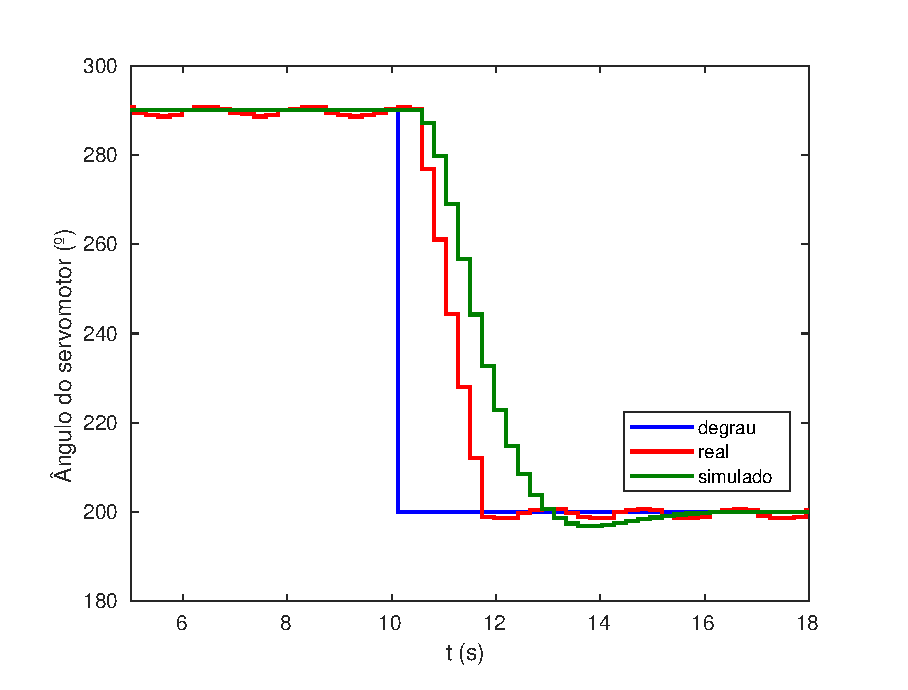
\includegraphics[width = 1\columnwidth]{Imagens/base_mf_simul}
    \fonte{Do autor}
    \label{fig:base_mf_simul}
  \end{subfigure}%
  \begin{subfigure}{.5\textwidth}
    \centering
    \caption{Ombro}
    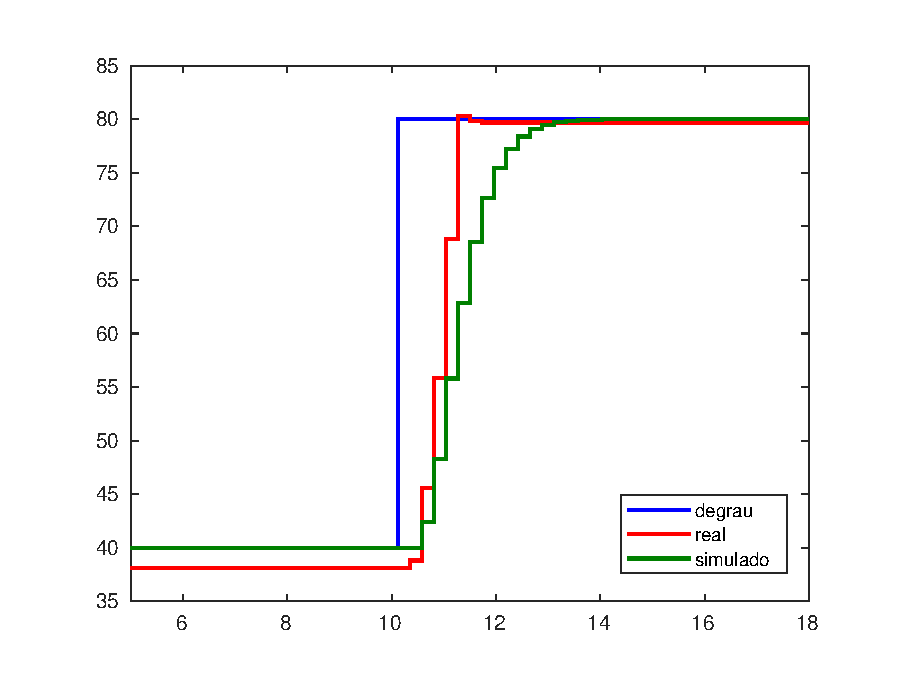
\includegraphics[width = 1\columnwidth]{Imagens/shoulder_mf_simul}
    \fonte{Do autor}
    \label{fig:shoulder_mf_simul}
  \end{subfigure}%
  \\[5ex]
  \begin{subfigure}{\textwidth}
    \centering
    \caption{Cotovelo}
    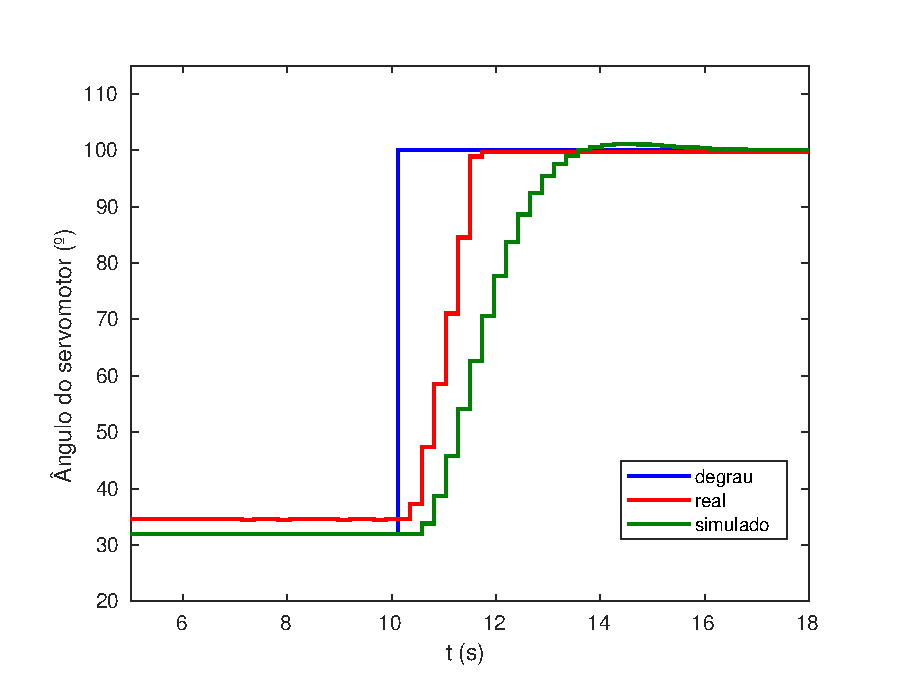
\includegraphics[width = 0.55\columnwidth]{Imagens/forearm_mf_simul}
    \fonte{Do autor}
    \label{fig:forearm_mf_simul}
  \end{subfigure}%
  
  \label{fig:ensaioMalhaAberta} 

\end{figure}

Com o primeiro controlador projetado para a base e para o cotovelo, ao fechar a malha, a resposta não apresentava
sobresinal como mostrado na \autoref{fig:base_mf_simul} e na \autoref{fig:forearm_mf_simul}. Apesar disso,
ao passar para o domínio discreto, o controlador passava a ter um zero não mínimo. E como foi citado 
anteriormente, o zero não mínimo é um comportamento indesejado para o sistema, por esse motivo, o controlador
de ambas as juntas foi alterado.

\section{Fase 2 da técnica HIL}
\markright{\thesection ~~~ Fase 2 da técnica HIL}

Como o sinal da resposta da planta sofre uma discretização ao comunicar com a placa de aquisição de dados do
computador e da \textit{Raspberry}, torna-se necessária a discretização do controlador e da planta simulada. A 
discretização foi feita através do comando \textit{c2d( )} do \textit{Matlab} através do método do segurador de 
ordem zero e com um tempo de amostragem de $0,23s$. O resultado para cada uma das juntas
segue abaixo respeitando a ordem de configuração do manipulador:

\begin{equation}
  \begin{gathered}
    G(z) = \frac{0,8273z - 0,6543}{z^2 - 0,9515z + 0,1245} \quad e \quad C(z) = \frac{0,152z + 0,032}{z - 1}
  \end{gathered}
  \label{eq:base_discrete}
\end{equation}

\begin{equation}
  \begin{gathered}
    G(z) = \frac{0,3876z - 0,198}{z^2 - 0,5515z + 0,1393} \quad e \quad C(z) = \frac{0,1572z + 0,06513}{z - 1}
  \end{gathered}
  \label{eq:shoulder_discrete}
\end{equation}

\begin{equation}
  \begin{gathered}
   G(z) = \frac{0,8273z - 0,6543}{z^2 - 0,9515z + 0,1245} \quad e \quad C(z) = \frac{0,152z + 0,032}{z - 1}
  \end{gathered}
  \label{eq:forearm_discrete}
\end{equation}

O próximo passo foi a obtenção da equação de diferenças para cada uma das plantas e
controladores.

\section{Resumo do Capítulo}
\markright{\thesection ~~~ Resultados}

% wn = 3.6522 / xi = 1 / ts = 1.0952s
% wn = 5.3571 / xi = 0.8 / ts = 0.9333s

Este capítulo apresentou de forma sucinta a metodologia de projeto a ser seguida para 
alcançar os objetivos propostos neste trabalho. No próximo capítulo são realizadas 
as modelagens cinemática e dinâmica do manipulador, a partir das quais o ambiente de 
simulação será construído.


\clearpage